% git mtm presentation

\documentclass{beamer}

\setbeamertemplate{navigation symbols}{}

\mode<presentation>
{
  \usetheme{Boadilla}
  % or ...

  %\setbeamercovered{transparent}
  % or whatever (possibly just delete it)
}

\usepackage{color}
\usepackage[english]{babel}
\usepackage[latin1]{inputenc}
\usepackage{times}
\usepackage[T1]{fontenc}
\usepackage{natbib}
\def\newblock{\hskip .11em plus .33em minus .07em}
\usepackage{fancybox}
\usepackage{hyperref}
% Or whatever. Note that the encoding and the font should match. If T1
% does not look nice, try deleting the line with the fontenc.

\title[Git MTM] % (optional, use only with long paper titles)
{Keeping track of computer work (e.g. R code) using Git}

\subtitle
{BIO R workshop series}

\author
{Clark Richards and Ryan Stanley}
% - Use the \inst{?} command only if the authors have different
%   affiliation.

% \institute[] % (optional, but mostly needed)
% {DAL}

\date% (optional)
{2017-10-06}

\subject{Talks}
% This is only inserted into the PDF information catalog. Can be left
% out. 



% If you have a file called "university-logo-filename.xxx", where xxx
% is a graphic format that can be processed by latex or pdflatex,
% resp., then you can add a logo as follows:

% \pgfdeclareimage[height=0.5cm]{university-logo}{figs/logos/cdogs_dal_logo.pdf}
% \logo{\pgfuseimage{university-logo}}

% Delete this, if you do not want the table of contents to pop up at
% the beginning of each subsection:
% \AtBeginSubsection[]
% {
%   \begin{frame}<beamer>{Outline}
%     \tableofcontents[currentsection,currentsubsection]
%   \end{frame}
% }


% If you wish to uncover everything in a step-wise fashion, uncomment
% the following command: 

%\beamerdefaultoverlayspecification{<+->}


\begin{document}

\begin{frame}
  \titlepage
\end{frame}

% \begin{frame}{Outline}
%   \tableofcontents
%   % You might wish to add the option [pausesections]
% \end{frame}

\begin{frame}[fragile]{R workshop topics}

  \begin{itemize}
  \item Git/RStudio
  \item R Basics
  \item packages and package development
  \item the \verb|oce| package
  \item the tidyverse
  \item ...?
  \end{itemize}

\end{frame}

\section{Is git useful for me?}

\begin{frame}{Is git useful for me?}

Do you ...
\begin{itemize}
\item<1-4> type text into a computer?
\item<2-4> hate losing (important) work?
\item<3-4> work from more than one computer?
\item<4> like knowing that your painstakingly written and brilliant
  code is backed up reliably?
\end{itemize}

\end{frame}

\begin{frame}

  Do you have folders like this?
  \begin{figure}
    \centering
    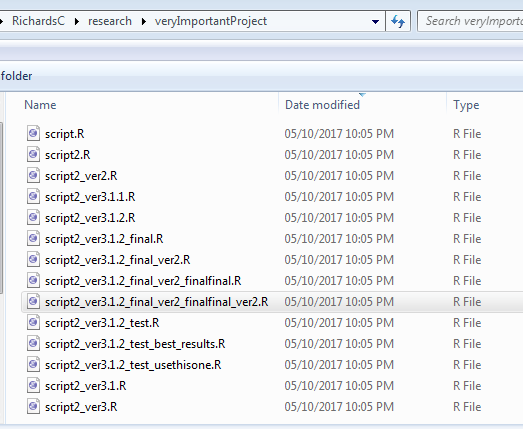
\includegraphics[height=0.9\textheight]{versioncontrol}
  \end{figure}

\end{frame}

\section{What is git?}

\begin{frame}{What is git?}

  Git is a free and open source, {\it distributed} {\bf version
    control} system designed to handle everything from small to very
  large projects with speed and efficiency (www.git-scm.com)
  \vspace{2em}
  \begin{itemize}
  \item {\bf Version Control:} keeps a history of everything you've
    done -- even files you've deleted.
  \item {\it Distributed:} Many people can work on the same project
    simultaneously without risk of losing work due to collisions
    (e.g. Linux kernel developers)
  \end{itemize}
\end{frame}

\section{How do I use it?}

\begin{frame}{Ways to use it}
    Using the software
    \begin{itemize}
        \item Terminal / command-line
        \item \textbf{RStudio}
        \item GitHub Desktop
        \item SourceTree
    \end{itemize}
    Hosting your repository
    \begin{itemize}
        \item Locally
        \item Github
        \item Bitbucket
        \item ...
    \end{itemize}
\end{frame}

\begin{frame}{How do I use it?}{\url{https://xkcd.com/1597/}}

  \begin{figure}
    \centering
    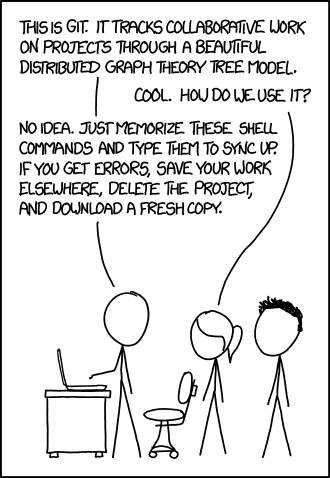
\includegraphics[height=0.8\textheight]{git}
  \end{figure}
  
\end{frame}

\begin{frame}[fragile]{How do I use it?}
  \begin{itemize}
  \item Create a repository (repo): \verb|git init|
  \item add files to the repo: \verb|git add file.txt|
  \item make changes to the file
  \item commit changes: \verb|git commit|
  \item When using ``remotes'' (e.g. Github), push changes: \verb|git push|
  \item repeat!
  \end{itemize}

\end{frame}

% \begin{frame}[fragile]
%     \begin{block}{Branching}
%         Helps keep track when things aren't linear in time.

%         Example uses:
%         \begin{itemize}
%             \item Collaborating (e.g. on a paper)
%             \item Experimenting / working on multiple things in parallel
%         \end{itemize}

%         \begin{verbatim}

% git checkout -b "paper-revisions"
% (make changes)
% git checkout master
% git merge paper-revisions

%         \end{verbatim}
%     \end{block}
% \end{frame}

\begin{frame}{
\includegraphics[width=0.4\textwidth]{github}}

  Github.com is one of the most popular cloud-based git repository hosting
  services. Basic accounts are free, which allows you to host as many
  \textbf{public} repos as you want. To have \textbf{private} repos,
  you need to either:
  \begin{itemize}
  \item pay money for a higher level account
  \item sign up for a Github education account 
  \end{itemize}

  \pause

  \begin{figure}
    \centering
    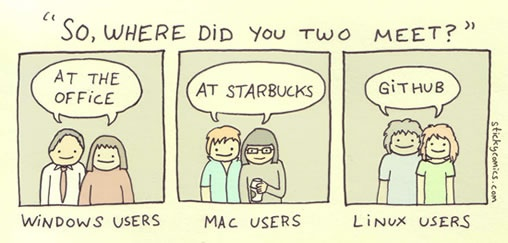
\includegraphics[width=0.7\textwidth]{comic1}
  \end{figure}
  
\end{frame}

\begin{frame}{Using Git through RStudio}

  \begin{figure}
    \centering
    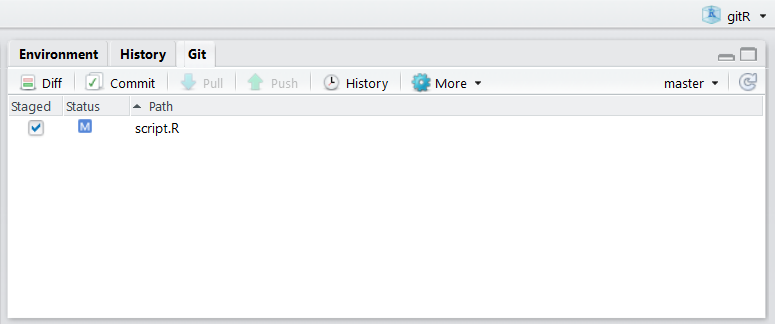
\includegraphics[width=\textwidth]{rstudiogit}
  \end{figure}

\end{frame}

\end{document}

%%% Local Variables:
%%% mode: latex
%%% TeX-master: t
%%% End:
